\documentclass[journal]{vgtc}                % final (journal style)
%\documentclass[review,journal]{vgtc}         % review (journal style)
%\documentclass[widereview]{vgtc}             % wide-spaced review
%\documentclass[preprint,journal]{vgtc}       % preprint (journal style)
%\documentclass[electronic,journal]{vgtc}     % electronic version, journal

%% Uncomment one of the lines above depending on where your paper is
%% in the conference process. ``review'' and ``widereview'' are for review
%% submission, ``preprint'' is for pre-publication, and the final version
%% doesn't use a specific qualifier. Further, ``electronic'' includes
%% hyperreferences for more convenient online viewing.

%% Please use one of the ``review'' options in combination with the
%% assigned online id (see below) ONLY if your paper uses a double blind
%% review process. Some conferences, like IEEE Vis and InfoVis, have NOT
%% in the past.

%% Please note that the use of figures other than the optional teaser is not permitted on the first page
%% of the journal version.  Figures should begin on the second page and be
%% in CMYK or Grey scale format, otherwise, colour shifting may occur
%% during the printing process.  Papers submitted with figures other than the optional teaser on the
%% first page will be refused.

%% These three lines bring in essential packages: ``mathptmx'' for Type 1
%% typefaces, ``graphicx'' for inclusion of EPS figures. and ``times''
%% for proper handling of the times font family.

\usepackage{mathptmx}
\usepackage{graphicx}
\usepackage{times}

%%% Algorithm packages added by J.P. (not in original template)
\usepackage{algorithm}
\usepackage[noend]{algpseudocode} % algorithm environment

%% We encourage the use of mathptmx for consistent usage of times font
%% throughout the proceedings. However, if you encounter conflicts
%% with other math-related packages, you may want to disable it.

%% This turns references into clickable hyperlinks.
\usepackage[bookmarks,backref=true,linkcolor=black]{hyperref} %,colorlinks
\hypersetup{
  pdfauthor = {},
  pdftitle = {},
  pdfsubject = {},
  pdfkeywords = {},
  colorlinks=true,
  linkcolor= black,
  citecolor= black,
  pageanchor=true,
  urlcolor = black,
  plainpages = false,
  linktocpage
}

%% If you are submitting a paper to a conference for review with a double
%% blind reviewing process, please replace the value ``0'' below with your
%% OnlineID. Otherwise, you may safely leave it at ``0''.
\onlineid{0}

%% declare the category of your paper, only shown in review mode
\vgtccategory{Research}

%% allow for this line if you want the electronic option to work properly
\vgtcinsertpkg

%% In preprint mode you may define your own headline.
%\preprinttext{To appear in an IEEE VGTC sponsored conference.}

%% Paper title.

\title{Subvolume Blocking with Direct Volume Rendering}

%% This is how authors are specified in the journal style

%% indicate IEEE Member or Student Member in form indicated below
\author{Jim Pelton}
\authorfooter{
%% insert punctuation at end of each item
\item
 Jim Pelton is with Boise State University. E-mail: jimpelton@boisestate.edu.
%\item
% Ed Grimley is with Grimley Widgets, Inc.. E-mail: ed.grimley@aol.com.
%\item
% Martha Stewart is with Martha Stewart Enterprises at Microsoft
% Research. E-mail: martha.stewart@marthastewart.com.
}

%other entries to be set up for journal
\shortauthortitle{Pelton \MakeLowercase{\textit{et al.}}: Subvolume Blocking with Direct Volume Rendering}
%\shortauthortitle{Firstauthor \MakeLowercase{\textit{et al.}}: Paper Title}

%% Abstract section.
\abstract{Duis autem vel eum iriure dolor in hendrerit in vulputate
velit esse molestie consequat, vel illum dolore eu feugiat nulla
facilisis at vero eros et accumsan et iusto odio dignissim qui blandit
praesent luptatum zzril delenit augue duis dolore te feugait nulla
facilisi. Lorem ipsum dolor sit amet, consectetuer adipiscing elit,
sed diam nonummy nibh euismod tincidunt ut laoreet dolore magna
aliquam erat volutpat. Ut wisi enim ad minim veniam, quis nostrud exerci tation ullamcorper
suscipit lobortis nisl ut aliquip ex ea commodo consequat. Duis autem
vel eum iriure dolor in hendrerit in vulputate velit esse molestie
consequat, vel illum dolore eu feugiat nulla facilisis at vero eros et
accumsan et iusto odio dignissim qui blandit praesent luptatum zzril
delenit augue duis dolore te feugait nulla facilisi.
} % end of abstract

%% Keywords that describe your work. Will show as 'Index Terms' in journal
%% please capitalize first letter and insert punctuation after last keyword
\keywords{Radiosity, global illumination, constant time}

%% ACM Computing Classification System (CCS). 
%% See <http://www.acm.org/class/1998/> for details.
%% The ``\CCScat'' command takes four arguments.

\CCScatlist{ % not used in journal version
 \CCScat{K.6.1}{Management of Computing and Information Systems}%
{Project and People Management}{Life Cycle};
 \CCScat{K.7.m}{The Computing Profession}{Miscellaneous}{Ethics}
}

%% Uncomment below to include a teaser figure.
  \teaser{
 \centering
 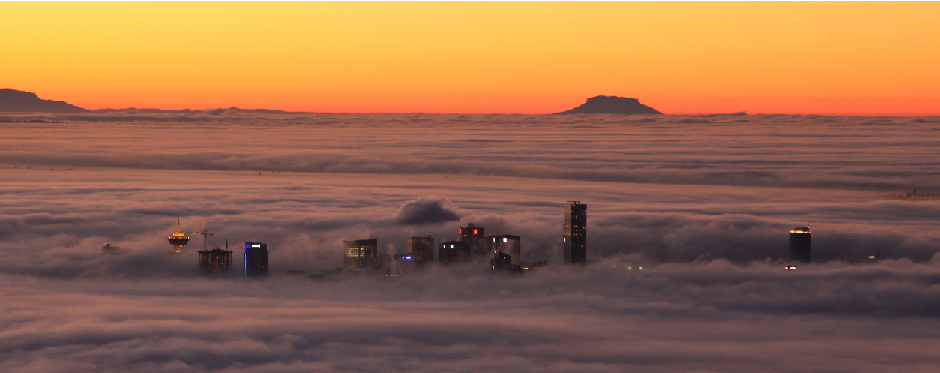
\includegraphics[width=16cm]{CypressView}
  \caption{In the Clouds: Vancouver from Cypress Mountain.}
  }

%% Uncomment below to disable the manuscript note
%\renewcommand{\manuscriptnotetxt}{}

%% Copyright space is enabled by default as required by guidelines.
%% It is disabled by the 'review' option or via the following command:
% \nocopyrightspace

%%%%%%%%%%%%%%%%%%%%%%%%%%%%%%%%%%%%%%%%%%%%%%%%%%%%%%%%%%%%%%%%
%%%%%%%%%%%%%%%%%%%%%% START OF THE PAPER %%%%%%%%%%%%%%%%%%%%%%
%%%%%%%%%%%%%%%%%%%%%%%%%%%%%%%%%%%%%%%%%%%%%%%%%%%%%%%%%%%%%%%%%

\begin{document}

%% The ``\maketitle'' command must be the first command after the
%% ``\begin{document}'' command. It prepares and prints the title block.

%% the only exception to this rule is the \firstsection command
\firstsection{Introduction}

\maketitle

%% \section{Introducction} %for journal use above \firstsection{..} instead
Direct volume rendering (DVR) is a visualization technique for the display of
3D scalar fields. It excels at rendering interior views of 3D scanned
objects, simulation data, or any subject lacking a well defined structure, such
as gaseous phenomena. However, a significant problem with DVR is that the
memory requirements of volume data sets quickly exceed the size of available
memory on the graphics processor.  When data exceeds available gpu memory, 
interactive visualization becomes impossible without using complex out-of-core 
rendering methods. 

Modern 3D scanning techniques and simulations produce enormous amounts of
three-dimensional data.  For example, the Biomolecular Research Institute at
Boise State University owns a micro-CT scanner that can generate high
resolution scans up to $8192^3$ voxels, producing approximately 2.2TB of
information.\footnote{Assuming the data set is represented using 32-bit
	floating point representation 
	($8192^3 = 512\textnormal{G}$, 
	and $4\textnormal{bytes/float} \times 8192^3 \approx 2.2\textnormal{TB}$).} 
The Idaho National Lab is also producing
high resolution scans of $2048^3$ voxels,
with each scan producing approximately 34.4GB of data.
Table~\ref{table:targetedDataSets} lists test data sets and sizes used for this
report.

The problem addressed by this project is that these real-world data sets are
too large to fit in the largest GPU memory capacities available today
(12--16GB).  Rendering these volumes requires complicated out-of-core methods that can
negatively impact visual quality and interactivity.  

\begin{table}[h]\label{table:targetedDataSets}
	 	 \caption{Selected data sets and dimensions ($1\textnormal{K}=\nobreak1024$) 
	 	 	with corresponding sizes in bytes.}
	 \scriptsize

	\begin{center}
		\begin{tabular}{lcc}
			\textbf{Data set} & \textbf{Dimensions} (voxels) & \textbf{Size} (bytes)\\
			\hline
			Hop flower & $512^3$ & $536$MB \\
			Graphite foam & $1\textnormal{K}^3$ & $4.3$GB  \\
			Bone fragment & $2\textnormal{K}^3$ & $34.4$GB  \\
			Synthetically generated volume & $4\textnormal{K}^3$ & $274.8$GB \\
			Synthetically generated volume & $8\textnormal{K}^3$ & $2.2$TB  \\
		\end{tabular}
	\end{center}
	
\end{table}

\section{Related Work}

\section{Methods}

%\subsection{Identifying empty data}
Volume data usually contains large, coherent regions where neighboring voxels
share similar properties. These regions will likely be assigned similar color
and opacity values. If the homogeneous regions are of no interest to the user
we can try to remove as many of these neighboring voxels as possible.
One way to do this is to split the volume data set into small 
subvolumes which can be classified as relevant or irrelevant. Classification
is done by visiting each voxel in a subvolume and using a user defined 
classifier to decide if the voxel is relevant or irrelevant. Subvolumes with a
user defined percentage of irrelevant voxels can be removed.

Rectangular subvolumes are used because 3D textures on the GPU cannot
be jagged---they must be rectangular 3D arrays of image data.

This project uses a classification scheme to identify the empty data. A user defined
classifier function that maps voxel values to voxel relevance is employed to identify
which space should be removed. 

It is prohibitively expensive to analyze each voxel for relevance. Prior to using the classifier,
the empty space removal procedure from~\cite{Vidal2008-dx} is used. 
They recursively shrink the bounding volume around regions of non-empty space
starting from the outside of the volume. The algorithm gains its efficiency by
using a summed volume table to compute the volume of candidate bounding
volumes. This allows culling large amounts of unneeded data very quickly from around 
the outsides of the useful data. However, the Vidal method is an outside-in approach. To
achieve fine grained data removal we utilize a second pass with our classification method.

\subsection{Basic subvolume blocking}\label{sec:basicSubvolumeBlocking}

Basic subvolume blocking divides the original volumetric data set into small,
uniformly sized subvolumes. Each subvolume is sent to the GPU
as an individual 3D texture (one texture is generated for each subvolume). 
Algorithm~\ref{alg:initGpuTexture}
shows the method for generating a small 3D texture, $T_{i,j,k}$ for a subvolume
$S_{i,j,k}$.

The basic approach does not reduce the size of the data on the GPU, but does
improve cache performance if the subvolumes are sized according to texture
cache size. In order to reduce the amount of data sent to the GPU we must have 
a way to determine which subvolumes are relevant to the visualization through
a classification process.


\begin{figure}[htb]\label{fig:volumeToSubvolumes}
	\begin{centering}
		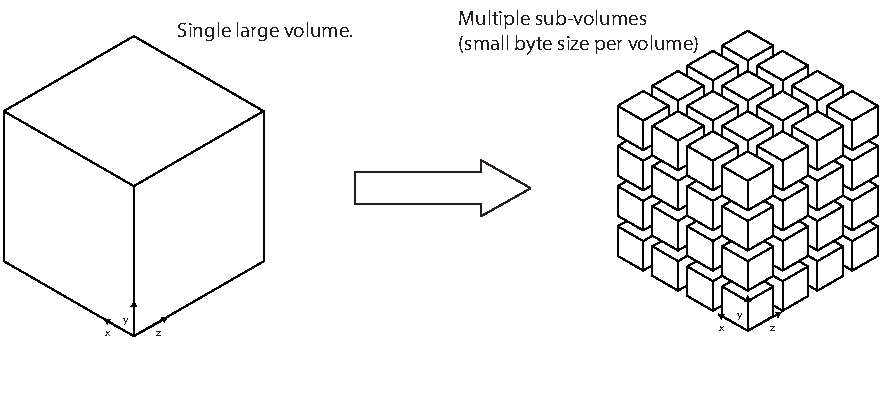
\includegraphics[width=\linewidth,height=0.3\textheight,keepaspectratio]{volume_to_subvolumes}
		\caption{Subvolume blocking splits the original data set into small subvolumes.}
	\end{centering}
\end{figure}

\begin{algorithm}[]  
	\begin{algorithmic}[1]
		\Procedure{InitGpuTexture}{i, j, k, V} 
		\State $T_{i,j,k} \gets $ \Call{alloc}{$S_x \times S_y \times S_z$} \Comment{Allocate tex buffer}
		\For{$s_w \gets 0 .. S_z$} \Comment{For each voxel in $S_{i,j,k}$}
		\For{$s_v \gets 0 .. S_y$}
		\For{$s_u \gets 0 .. S_x$} 
		\State $u \gets s_u + i \times S_x$ \Comment{Compute offsets into V}
		\State $v \gets s_v + j \times S_y$ 
		\State $w \gets s_w + k \times S_z$ 
		\State $T_{i,j,k}\left[s_u, s_v, s_w \right] \gets V\left[u,v,w\right]$ \Comment{Copy to texture buffer}
		\EndFor
		\EndFor
		\EndFor
		\EndProcedure
	\end{algorithmic}
	\caption{Initialize texture $T_{i,j,k}$ for subvolume $S_{i,j,k}$.}
	\label{alg:initGpuTexture}
\end{algorithm}


\subsection{Subvolume blocking with classification}\label{sec:subvolumeBlockingWithClassification}

To facilitate easy data removal, the basic subvolume blocking approach can be extended to 
include a classification step that identifies subvolumes relevant to the desired visualization. 
\textit{Relevant} subvolumes are expected to contribute in some way to the visualization, otherwise 
a subvolume is \textit{irrelevant}. Algorithm~\ref{alg:partitionAndThreshold} shows how the classification 
step is merged  with the basic subdivision algorithm (Algorithm~\ref{alg:initGpuTexture}).

Determining if a subvolume is relevant requires examining each voxel in the
volume to determine the voxel relevance. The user must supply the classifier
function, the minimum voxel relevance threshold, and a total relevant voxel
threshold. If the number of relevant voxels in the subvolume is above the total
relevant voxel threshold then the subvolume is relevant to the visualization.
Algorithm~\ref{alg:threasholdSubVolume} shows one way to determine subvolume
relevance from a voxel classifier ($C_{r}$), classification threshold ($t_{min}$),
and the relevant voxel threshold ($s_{min}$).

\begin{algorithm}[]
	\begin{algorithmic}[1]  
		\Procedure{PartitionAndThreshold}{$V$}
		\For{$i\gets 0 .. N_x$} \Comment{For each subvolume}  
		\For{$j\gets 0 .. N_y$}   
		\For{$k\gets 0 .. N_z$}   
		\If{\textit{subvolume i,j,k is relevant}} 
		\State \Call{InitGpuTexture}{i, j, k, V} \Comment{Send to GPU}
		\EndIf
		\EndFor
		\EndFor
		\EndFor
		\EndProcedure
	\end{algorithmic}
	\caption{Partition $V$ into subvolumes with thresholding.}
	\label{alg:partitionAndThreshold}
\end{algorithm}



\begin{algorithm}[]
	\begin{algorithmic}[1]
		\Procedure{IsSubvolumeRelevant}{$S_{i,j,k}, C_{r}, t_{min}, s_{min}$}
		\State $sum \gets 0$  \Comment{Relevant voxels found so far.}
		
		\ForAll{voxels in $S_{i,j,k}$}
		
		\State $r \gets$ \textit{voxel relevance from $C_{r}$} \Comment{Run classifier on voxel.}
		\If{\textit{$r > t_{min}$}} 
		\State $sum \gets sum + 1$  \Comment{Voxel is relevant}
		\EndIf
		\EndFor
		
		\If{\textit{$sum > s_{min}$}}
		\State \Return true \Comment{$S_{i,j,k}$ is relevant}
		\Else
		\State \Return false \Comment{$S_{i,j,k}$ is irrelevant}
		\EndIf
		\EndProcedure
	\end{algorithmic}
	\caption{Determine if $S_{i,j,k}$ is relevant to the visualization. $C_r$ is the classifier function,
		$t_{\min}$ is the classification threshold, and $s_{\min}$ is the relevant voxel threshold.}
	\label{alg:threasholdSubVolume}
\end{algorithm}

%\paragraph{Rejected Ejector Seat Reservation}
\section{Results}


\section{Conclusion}

%% if specified like this the section will be committed in review mode
\acknowledgments{
The authors wish to thank A, B, C. This work was supported in part by
a grant from XYZ.}

\bibliographystyle{abbrv}
%%use following if all content of bibtex file should be shown
%\nocite{*}
\bibliography{template}
\end{document}
